\chapter{I$^2$C Configuration}
\label{chap:I2C}

This chapter describes all necessary steps to get the two I$^2$C buses of the Raspberry Pi (Model B+) up and running. Because of different operating modes of the devices using the I$^2$C-Bus the usage of both buses is necessary.\newline\newline
%\textbf{HINT: These steps are not necessary if you install the Rasbian Image of the project. Within that image, everything should be configured.}\newline
HINT: These steps are not necessary if you install the Rasbian Image of the project. Within that image, everything should be configured.


\section{raspi-config}
\label{sec:raspiconfig}
Enable I$^2$C using raspi-config utility.\\\\
From the command line type:\\\\
\ttfamily \textbf{sudo raspi-config}\\\\
\normalfont This will open the raspi-config utility.

\begin{figure}[H]
	\centering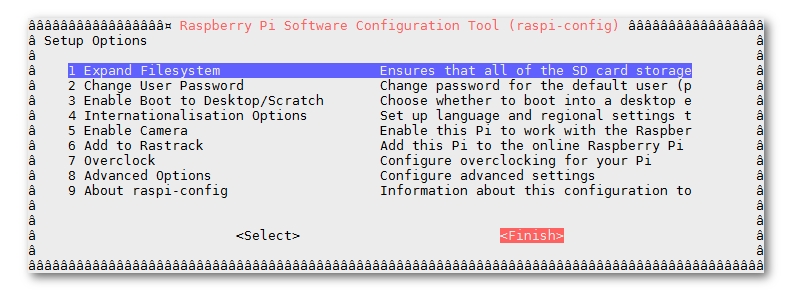
\includegraphics[width=\textwidth]{fig/raspi_config}
	\caption{raspi-config}
	\label{fig:raspiconfig}
\end{figure}

\newpage
\textbf{Now complete the following steps:}\\\\
Select: "8 - Advanced Options"\\
Select: "A7 - I$^2$C"\\
Select: "Yes"\\
The Screen will ask if you want the interface to be enabled:\\
Select: "Yes"\\
Select: "OK"\\
The Screen will ask if you want the module to be loaded by default:\\
Select: "Yes"\\
The Screen will state the module will be loaded by default:\\
Select: "OK"\\
Select "Finish" to return to the command line \\
When you next reboot the I$^2$C module will be loaded.\\


\section{Module File}
\label{sec:modulefile}
Next we need to edit manually the modules file using:\\
\ttfamily \textbf{sudo nano /etc/modules}\\
\normalfont and add the following lines:\\
\ttfamily \textbf{i2c-bcm2708\\
									i2c-dev}\\
\normalfont									
Use CTRL-X, then Y, then RETURN to save the file and exit.								





\section{I$^2$CTools}
\label{sec:I2Ctools}

For hardware monitoring, device identification, and troubleshooting we install "i2c-tools".\\\\
\ttfamily \textbf{sudo apt-get update\\
									sudo apt-get install i2c-tools}\\\\
\normalfont
Now shutdown your system, disconnect the power to your Pi and you are ready to connect your I$^2$C-Hardware.\\									


\section{Test I$^2$C-1}
\label{sec:testi2c1}

\textbf{Check if I$^2$C is enabled:}\\\\
When you power up or reboot your Pi you can check the I$^2$C module is running by using the following command:\\
\ttfamily \textbf{lsmod $|$ grep i2c\_}\\
\normalfont
That will list all the modules starting with "i2c\_". If it lists "i2c\_bcm2708" then the module is running correctly.\\\\

\textbf{Testing Hardware:}\\
Once you've connected your hardware double check the wiring. Make sure 5V is going to the correct pins and you've got not short circuits. Power up the Pi and wait for it to boot.\\
Then type the following command:\\\\
\ttfamily \textbf{sudo i2cdetect -y 1}\\\\
\normalfont 
With e.g. a sensor connected the output looks e.g. like this:\\

\ttfamily
 \quad\quad  0  1  2  3  4  5  6  7  8  9  a  b  c  d  e  f \\
00:\qquad\quad\quad-- -- -- -- -- -- -- -- -- -- -- -- -- \\
10: -- -- -- -- -- -- -- -- -- -- -- -- -- -- -- -- \\
20: -- -- -- -- -- -- -- -- -- -- -- -- -- -- -- -- \\
30: -- -- -- -- -- -- -- -- -- -- -- -- -- -- -- -- \\
40: -- -- -- -- -- -- -- -- -- -- -- -- -- -- -- -- \\
50: -- -- -- -- -- -- -- -- -- -- -- -- -- -- -- -- \\
60: -- -- 62 -- -- -- -- -- -- -- -- -- -- -- -- -- \\
70: -- -- -- -- -- -- -- -- \\\\
\normalfont

This shows that one device is connected and its address is 0x62.\\ 


\newpage

\section{Set up I$^2$C-0}
\label{sec:setupi2c0}


In normal configuration the second I$^2$C-Bus of the Raspberry Pi is set up as two of the output pins of the DSI Display Connector resp. the CSI Camera Connector.\\
To make the setup of the quadrocopter as easy as possible and with respect to the weight and soldering/cabling these output pins were redirecteed to two of the 40 pins of the GPIO Header.\\

This gets done by useage of a Python-script (see below) which gets excecuted while booting the system. To get this configuration running two additional files need to be edited.\\\\
In "/boot/cmdline.txt"\\
\ttfamily bcm2708.vc\_i2c\_override=1 \\
\normalfont has to be added\\
in "/etc/modprobe.d/i2c\_o\_enable.conf"\\
\ttfamily{blacklist snd\_soc\_tas5713} \\
\normalfont has to be added.\\

After this the GPIO port 27 is configured as SDA0 and the GPIO port 28 as SCL0.

\begin{figure}[H]
	\centering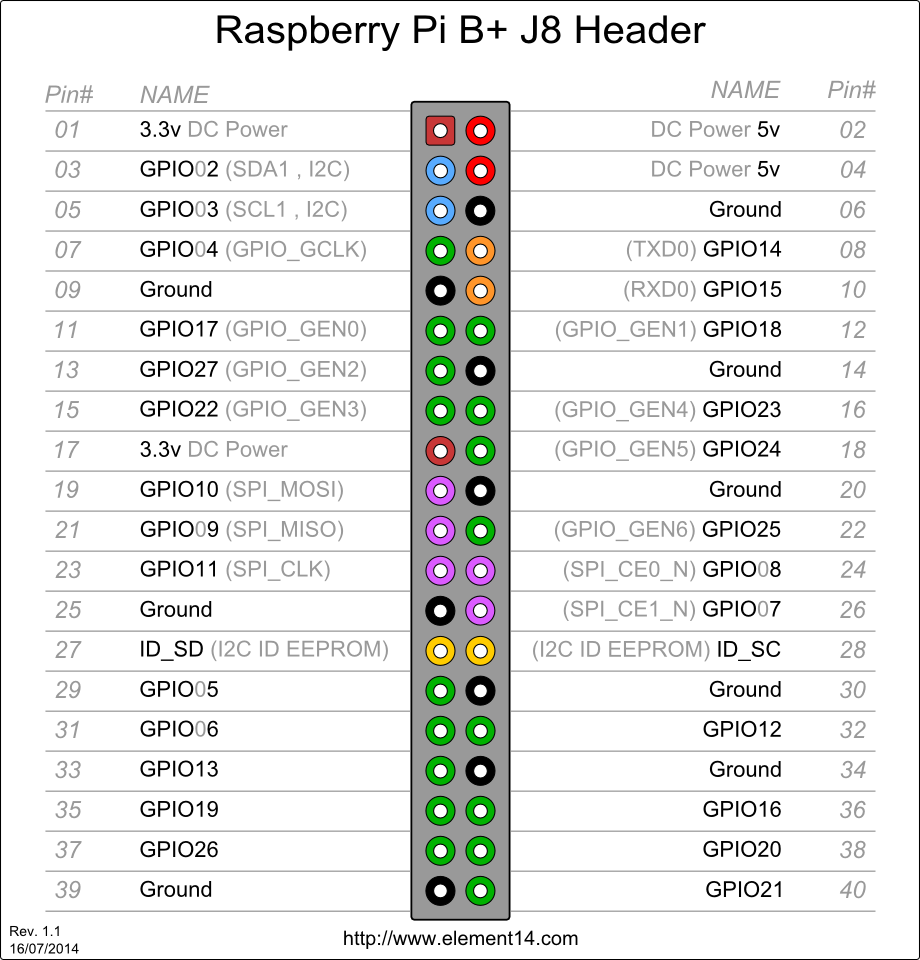
\includegraphics[width=0.5\textwidth]{fig/gpios}
	\caption{GPIOs \footnotemark}
	\label{fig:gpios}
\end{figure}
\footnotetext{\url{http://www.element14.com/community/servlet/JiveServlet/previewBody/68203-102-6-294412/GPIO.png}}
\newpage


\lstinputlisting[language=Python, basicstyle=\tiny, caption=I$^2$C0 Port-Configuration]{add_files/I2C0_Config_OS.py}




